\section*{Schema di principio}
\begin{figure}[H]
    \centering
    \includegraphics[width=0.7\textwidth]{example-image}
    \caption{Schema di principio del circuito.}
\end{figure}
\newpage

\section{Schema planimetrico}
\begin{figure}[H]
    \centering
    \includegraphics[width=0.7\textwidth]{example-image}
    \caption{Schema planimetrico del montaggio con i componenti.}
\end{figure}

\section{Strumenti, attrezzature e componenti utilizzati}
\begin{table}[H]
\centering
\rowcolors{2}{lightgray}{white}
\begin{tabular}{@{}|ll|@{}}
\toprule
\textbf{Categoria} & \textbf{Descrizione} \\ \midrule
Breadboard & Piastra sperimentale  \\
Resistenze & \SI{10}{\kilo\ohm}, \SI{100}{\ohm} \\
Generatore di segnali & Generatore di funzioni n ABCXYZ \\
Oscilloscopio digitale & Strumento XYZABC\\
Multimetro & Misuratore universale di tensione, corrente e resistenza \\
OpAmp 741 & Amplificatore operazionale universale \\ \bottomrule
\end{tabular}
\caption{Strumenti, attrezzature e componenti utilizzati}
\end{table}

\section{Procedimento}
\begin{enumerate}
    \item Montaggio del circuito secondo lo schema di principio.
    \item Collegamento degli strumenti di misura.
    \item Impostazione del generatore di segnale.
    \item Rilevazione dei valori con multimetro e oscilloscopio.
    \item Registrazione e analisi dei dati.
\end{enumerate}

\section{Tabelle dei dati e calcoli}
\begin{table}[H]
\centering
\rowcolors{2}{lightgray}{white}
\begin{tabular}{@{}|c|c|c|c|@{}}
\toprule
$V_{in}$ (V) & $V_{out}$ (V) & Rapporto $\frac{V_{out}}{V_{in}}$ & Osservazioni \\ \midrule
0.1 & -1.0 & -10.0 & Lineare \\
0.2 & -2.0 & -10.0 & Lineare \\
0.5 & -5.1 & -10.2 & Saturazione \\ \bottomrule
\end{tabular}
\caption{Dati sperimentali con calcoli effettuati.}
\end{table}

\section{Grafico}
\begin{figure}[H]
\centering
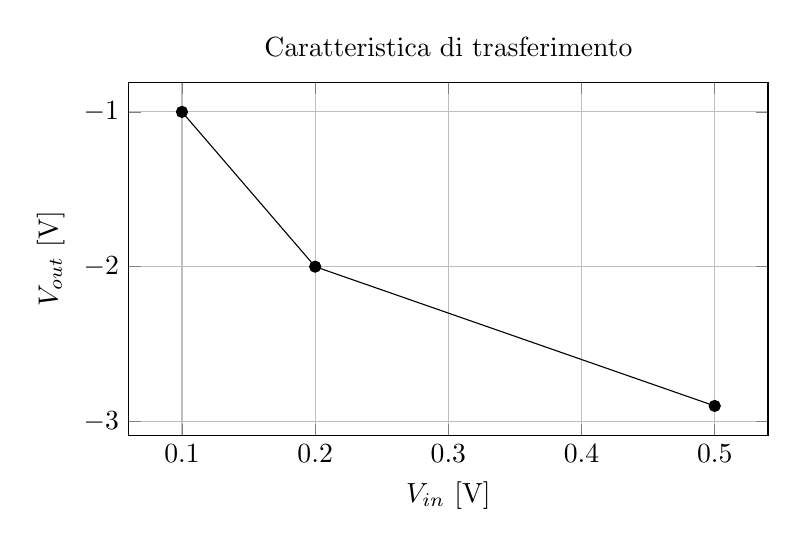
\begin{tikzpicture}
\begin{axis}[
    title={Caratteristica di trasferimento},
    xlabel={$V_{in}$ [V]},
    ylabel={$V_{out}$ [V]},
    grid=major,
    width=0.8\textwidth,
    height=0.5\textwidth
]
\addplot[color=black, mark=*] coordinates {
    (0.1,-1.0)
    (0.2,-2.0)
    (0.5,-2.9)
};
\end{axis}
\end{tikzpicture}
\caption{Grafico della caratteristica di trasferimento.}
\end{figure}

\section{Conclusione}
Sintesi dei risultati ottenuti e confronto con la teoria.  
Commentare eventuali discrepanze, cause di errore e possibili miglioramenti.

\section{Utilizzo degli strumenti e valutazione dei rischi della prova}
\subsection{Misure da adottare}
Descrivere le precauzioni e le corrette procedure di sicurezza in laboratorio.
